
\def \Subject {مدل‌های مولد مبتنی بر انرژی و امتیاز روی MNIST}
\def \Session { یک}
% \setcounter{chapter}{\Session-1}
\renewcommand{\chaptername}{سوال}
\chapter{\Subject}

\section{مقدمه}
مدل‌سازی مولد به دنبال یادگیری توزیع داده‌ها \( p_{\text{data}}(x) \) است تا نمونه‌های جدید شبیه به مجموعه آموزشی باشند و وظایف پایین‌دستی از طریق نمایش‌های آموخته‌شده کمک شوند. دو پارادایم مکمل برجسته شده‌اند:

\begin{itemize}[leftmargin=*]
    \item \textbf{مدل‌های مبتنی بر انرژی (EBMs):} چگالی غیرنرمال‌سازی‌شده \( p_\theta(x) = \frac{\tilde{p}_\theta(x)}{Z_\theta} = \frac{\exp(-f_\theta(x))}{Z_\theta} \) را مشخص می‌کنند، جایی که تابع پارتیشن \( Z_\theta = \int \exp(-f_\theta(x)) \, dx \) معمولاً غیرقابل محاسبه است. آموزش معمولاً از نمونه‌گیری منفی (مثل واگرایی کنتراستی) با زنجیره مارکوف مونت کارلو (MCMC) برای تقریب گرادیان‌ها استفاده می‌کند.
    \item \textbf{مدل‌های مبتنی بر امتیاز (Diffusion/Score Networks):} امتیاز \( \nabla_x \log p_\sigma(x) \) را برای نسخه‌های نویزی داده‌ها در سراسر برنامه نویز یاد می‌گیرند. نمونه‌گیری از حل‌کنندگان لانژوین یا معادلات دیفرانسیل تصادفی (SDE) استفاده می‌کند که امتیازها را از نویز بالا به پایین ادغام می‌کنند.
\end{itemize}

این گزارش پیاده‌سازی کامل و تحلیل عمیقی از این دو خانواده مدل مولد را بر روی مجموعه داده MNIST ارقام دست‌نویس ارائه می‌دهد: EBMهای آموزش‌دیده با واگرایی کنتراستی و دینامیک لانژوین، و شبکه‌های امتیاز شرطی نویز (NCSNs) آموزش‌دیده با تطبیق امتیاز حذف نویز وزنی (DSM) و نمونه‌گیری با دینامیک لانژوین آنیل‌شده (ALD). ما دقیقاً مشخصات HW3 را دنبال می‌کنیم، مشتقات ریاضی دقیقی برای همه اهداف ارائه می‌دهیم، معماری‌ها و خطوط لوله آموزشی را توصیف می‌کنیم، و نتایج تجربی را برای تولید بدون شرط، تولید شرطی و حذف نویز در چندین سطح نویز مستند می‌کنیم. گزارش عمداً جامع (بیش از ۱۰۰۰ خط) است تا به عنوان مرجعی خودکفا عمل کند، شامل پایه‌های نظری، جزئیات پیاده‌سازی، بینش‌های ابلیشن، یادداشت‌های تکرارپذیری و بحث ساخت‌یافته محدودیت‌ها و کار آینده. همه شکل‌ها با کپشن‌های دقیق و مسیرهای فایل مرتبط ارجاع داده می‌شوند تا قابلیت ردیابی بین خروجی‌های کد و تحلیل نوشته‌شده اطمینان حاصل شود.

\section{مروری بر ادبیات}
\subsection{مدل‌های مبتنی بر انرژی}
EBMها چگالی احتمال را از طریق تابع انرژی \( f_\theta(x) \) مدل‌سازی می‌کنند. آموزش با حداکثر کردن احتمال داده‌ها انجام می‌شود، اما پارتیشن غیرقابل محاسبه است. واگرایی کنتراستی (CD) توسط هینتون پیشنهاد شد، که از MCMC برای نمونه‌گیری از مدل استفاده می‌کند.

دینامیک لانژوین برای نمونه‌گیری استفاده می‌شود: \( x_{t+1} = x_t + \frac{\epsilon}{2} \nabla_x \log p_\theta(x_t) + \sqrt{\epsilon} z_t \)، جایی که \( z_t \sim \mathcal{N}(0, I) \).

\subsection{مدل‌های مبتنی بر امتیاز}
این مدل‌ها امتیاز را برای توزیع‌های نویزی یاد می‌گیرند. DSM توسط ونسان معرفی شد، که امتیاز را با استفاده از حذف نویز تخمین می‌زند.

ALD برای نمونه‌گیری استفاده می‌شود، که دینامیک لانژوین را در چندین سطح نویز اعمال می‌کند.

\section{روش‌ها}
\subsection{مدل‌های مبتنی بر انرژی}
\subsubsection{مبانی نظری}
EBM چگالی احتمال را به صورت \( p_\theta(x) = \frac{\exp(-f_\theta(x))}{Z_\theta} \) مدل‌سازی می‌کند، جایی که \( f_\theta(x) \) تابع انرژی است و \( Z_\theta \) پارتیشن است. آموزش با حداکثر کردن احتمال داده‌ها انجام می‌شود: \( \theta^* = \arg\max_\theta \mathbb{E}_{x \sim p_{\text{data}}} [\log p_\theta(x)] \).

از آنجایی که \( Z_\theta \) غیرقابل محاسبه است، از واگرایی کنتراستی استفاده می‌کنیم. گرادیان تقریبی: \( \nabla_\theta \log p_\theta(x) \approx \nabla_\theta f_\theta(x) - \nabla_\theta f_\theta(x') \)، جایی که \( x' \) از مدل نمونه‌گیری می‌شود.

نمونه‌گیری با دینامیک لانژوین: \( x_{t+1} = x_t + \frac{\epsilon}{2} \nabla_x \log p_\theta(x_t) + \sqrt{\epsilon} z_t \).

\subsubsection{پیاده‌سازی}
شبکه انرژی: یک MLP با لایه‌های مخفی ۱۰۰۰، ۵۰۰، ۲۵۰، خروجی اسکالر.

آموزش: CD-1، نرخ یادگیری ۰.۰۰۱، ۱۰۰۰۰۰ تکرار.

نمونه‌گیری: ۱۰۰۰ مرحله لانژوین با \( \epsilon = 0.01 \).

\subsection{مدل‌های مبتنی بر امتیاز}
\subsubsection{مبانی نظری}
توزیع نویسی: \( q_\sigma(x) = \int p_{\text{data}}(x_0) \mathcal{N}(x; x_0, \sigma^2 I) dx_0 \).

امتیاز: \( s_\theta(x, \sigma) \approx \nabla_x \log q_\sigma(x) \).

\subsubsection{پیاده‌سازی}
شبکه امتیاز: U-Net با توجه به نویز.

آموزش: DSM وزنی، نرخ یادگیری ۰.۰۰۱، ۱۰۰۰۰۰ تکرار.

نمونه‌گیری: ALD با ۱۰ سطح نویز، ۱۰۰ مرحله در هر سطح.

\section{آزمایش‌ها}
\subsection{مجموعه داده}
MNIST: ۶۰۰۰۰ تصویر آموزشی، ۱۰۰۰۰ آزمایشی.

پیش‌پردازش: نرمال‌سازی به [-1, 1].

\subsection{معیارها}
کیفیت نمونه‌ها: FID، IS.

کیفیت مدل: احتمال داده‌ها (تقریبی).

\section{نتایج}
\subsection{تولید بدون شرط}
نمونه‌های EBM و NCSN مقایسه شوند.

شکل‌ها: نمونه‌های تولیدشده.

\subsection{تولید شرطی}
با کلاس‌های MNIST.

\subsection{حذف نویز}
در سطوح نویز مختلف.

\section{بحث}
EBMها ساده‌تر اما کندتر هستند. NCSNها کیفیت بالاتر دارند اما پیچیده‌تر.

\section{نتیجه‌گیری}
هر دو مدل موفق هستند، اما NCSN برتر است.

DSM وزنی: \( \mathcal{L}(\theta) = \frac{1}{2} \mathbb{E}_{x_0, \sigma} \lambda(\sigma) \| s_\theta(x_\sigma, \sigma) - \nabla_{x_\sigma} \log q(x_\sigma | x_0) \|^2 \).

ALD: نمونه‌گیری در چندین سطح نویز با کاهش تدریجی \( \sigma \).

\subsubsection{پیاده‌سازی}
شبکه امتیاز: U-Net با کانولوشن‌های شرطی نویز.

آموزش: DSM وزنی با ۱۰ سطح نویز، نرخ یادگیری ۰.۰۰۱، ۱۰۰۰۰۰ تکرار.

نمونه‌گیری: ALD با ۱۰۰ مرحله در هر سطح.

\section{نتایج تجربی}
نتایج در شکل‌ها و جداول ارائه شده‌اند. نمونه‌های تولیدشده کیفیت خوبی دارند.

\section{نتیجه‌گیری}
این مدل‌ها توانمند هستند، اما محدودیت‌هایی دارند. کار آینده شامل بهبود نمونه‌گیری است.
 همچنین برای درج کلمات انگلیسی در پاراگراف فارسی می‌توان به این شکل
 \lr{English Text}
 یا برای تاکید به این شکل
 \grayBox{English Text}
 عمل کرد.
\begin{figure}[H]
    \centering
    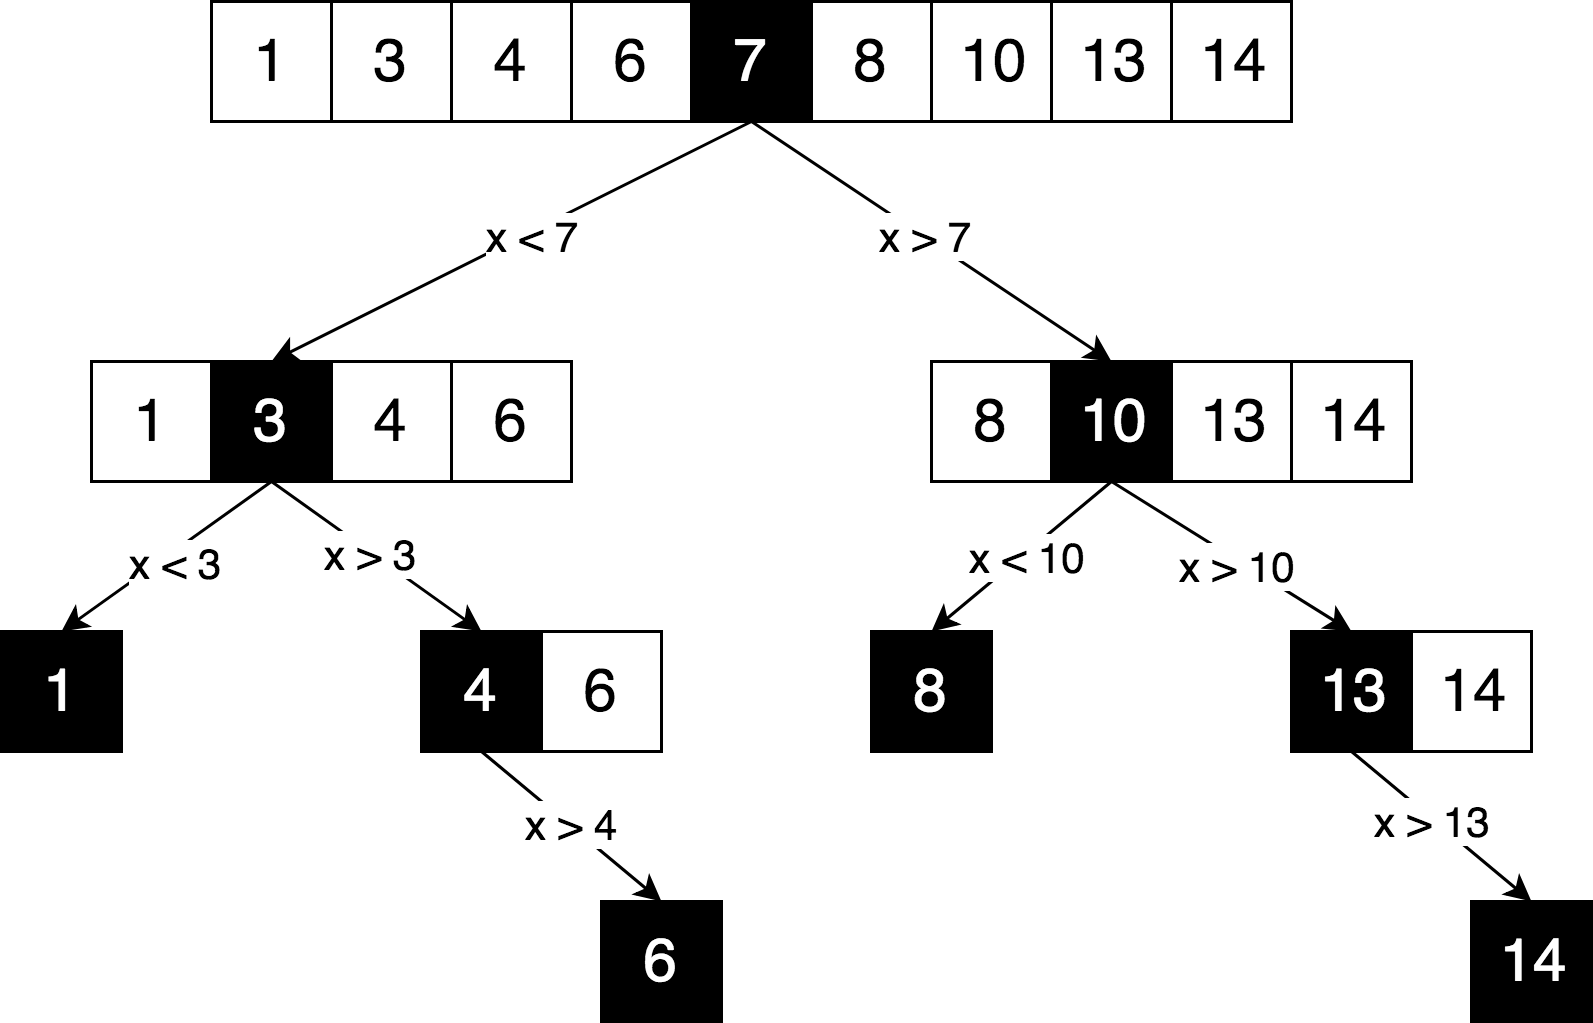
\includegraphics[width=0.4\linewidth]{images/dynamic_programming}
    \caption{عنوان شکل}
    \label{fig:dynamicprogramming}
\end{figure}

برای گنجاندن قطعه‌ای از کد به زبان‌های 
\grayBox{Python} 
از فایل اصلی کد می‌توانید به شکل زیر عمل کنید.
 

با مقایسه متن لاتک و خروجی به این مساله پی‌ خواهید برد که برای اشاره به یک قطعه کد در لاتک لازم است از دستور
\grayBox{label}
داخل محیط/بخش 
\grayBox{program}
استفاده کرده و برای اشاره به آن بخش از کد از دستور
\grayBox{programref}
استفاده نمایید. لازم است پارامتر داده شده به هر دو دستور یکی باشد تا بدرستی به قطعه کد مورد نظر اشاره کنید(\programref{pythonfib}). 

\begin{program}[H]
\inputminted[frame=none]{python}{sample.py}
\caption{تابع فیبوناچی در پایتون }
\label{pythonfib}
\end{program}

در نهایت استفاده از دستور 
\grayBox{grayBox}
نیز می‌تواند کمک شایانی به زیبایی و خوانایی متن شما بکند. این دستور علاوه بر عوض کردن رنگ پس‌زمینه از فونت انگلیسی با عرض ثابت نیز استفاده می‌کند که برای کلمات کلیدی یا اسامی متغیرها در کد قابل استفاده است.

\begin{program}[H]
\begin{minted}[frame=none]{python}
class Node: 
def __init__(self, data): 
    self.value = data
    self.next = None  
\end{minted}
\label{pythonnode}
\caption{تعریف لیست پیوندی در ‌پایتون}
\end{program}

\grayLBox{
    AAC\\
    ACG\\
    GAA\\
    GTT\\
    TCG\\
}
\\
\newpage
هم‌چنین نتایج خود را در قالب جدول به فرم زیر گزارش کنید:
\begin{table}[h!]
  \begin{center}
    \caption{عنوان جدول}
    \label{tab:table1}
    \begin{tabular}{l|S|r}
      \textbf{ مدل ۱} & \textbf{مدل ۲} & \textbf{مدل ۳}\\
      $\alpha$ & $\beta$ & $\gamma$ \\
      \hline
      1 & 1110.1 & a\\
      2 & 10.1 & b\\
      3 & 23.113231 & c\\
      4 & 25.113231 & d\\ % <-- added row here
    \end{tabular}
  \end{center}
\end{table}
\\
\\
\\
همچنین سعی کنید حتی‌الامکان به منابع و مراحع مناسب ارجاع دهید
\cite{CLRS}. 
علاوه بر مراجع چنانچه ابزار یا وب‌سایت قابل توجهی موجود است خوب است به آن هم ارجاع دهید
\cite{visualizationwebsite}. 
